\problemname{Mountain Parties}
Bergaburgir is a town located on a mountain.
In the town there are $M$ people and $N$ houses.
The people are numbered $1$ to $M$ and the houses $1$ to $N$.
Each house can have at most one resident.
Some houses may be empty, but every person lives in exactly one house.
Since it takes a long time to walk on the mountain, there is a slide from each house to another house further down the mountain (except the lowest house).

Up on a mountain there is not much to do, so the villagers have invented customs.
These customs have spiraled a bit out of control, and the villagers need your help to continue their traditions.

The first custom is relatively simple, but not always desirable.
It is that the villagers decide that the inhabitants (if there are any) of two houses should swap houses.
This is done by choosing two houses, $a$ and $b$.
If a person lives in house $a$, they are forced to move to house $b$.
Likewise, if a person lives in house $b$, they are forced to move to house $a$.

The second activity is hosting parties, which is significantly more complicated.
The goal of each party is of course to invite as many people as possible.
This is limited by the geography of the mountain and the strange friendship circles on the mountain.
Each person knows exactly two other people.
More precisely, person $i$ knows person $i-1$ and person $i+1$.
This is cyclic, so person $1$ knows persons $2$ and $M$.
Similarly, person $M$ knows persons $M-1$ and $1$.
In other words, the graph of friendships forms a cycle.

For a party to take place, a person $p$ must first volunteer as the host.
That person then decides how fun the party will be, denoted by $R$.
Then they may choose any house they want to hold the party in.
They may choose any house they wish.
Then the guests must be invited.
They first decide the number of guests including themselves, $K$ ($K \leq M$).
Then they tell exactly one of their friends that they are invited, and tell them to invite $K-1$ friends.
That friend in turn invites the only one of their friends who has not yet been invited, and tells them to invite $K-2$ friends.
This process continues until exactly $K$ people are invited, including the host.
Thus, the invited people form an interval of size $K$ along the friendship cycle, with the host at one of the endpoints.
For the party not to become a disaster, these people must be able to get to the party house.
For a person to be able to get to the party, they must be able to reach it by taking at most $R$ slides, where $R$ is the party's fun value.

Your task is now to determine the maximum number of people that can be invited to each party if the host plans it optimally.
Of course, you must also account for all house swaps.

\section*{Input}
The first line of input contains the integers $N$, $M$, and $Q$ ($1 \leq N, M, Q \leq 10^5$, $M \leq N$),
the number of houses, the number of inhabitants, and the number of customs performed.

The second line contains $N$ integers $r_1, \dots, r_N$ ($1 \leq r_i \leq N$),
where $r_i$ means that house $i$ has a slide to house $r_i$.
There is exactly one house where $r_i = i$, and this means that this house is the lowest and does not have a slide.
It is guaranteed that the slides form a tree rooted at the house where $r_i = i$.

The third line contains $M$ integers $h_1, \dots, h_M$ ($1 \leq h_i \leq N$),
where $h_i$ means that person $i$ lives in house $h_i$.
It is guaranteed that no two people live in the same house.

The final $Q$ lines each describe a custom being performed. Each line begins with the integer $T$ ($1 \leq T \leq 2$).

If $T=1$, a house swap has occurred. Then two integers $a$ and $b$ follow ($1 \leq a, b \leq N$, $a \neq b$),
which means that the inhabitants of houses $a$ and $b$ swap.

If $T=2$, a villager wants help planning a party. Then two integers $p$ and $R$ follow ($1 \leq p \leq M$, $1 \leq R < N$),
which means that person $p$ wants to host a party with fun value $R$.

\section*{Output}
For each query where $T=2$, output an integer: the maximum number of people who can be invited to a party
if person $p$ is the host and the party has fun value $R$.

\section*{Scoring}
Your solution will be tested on a set of test groups.
To earn points for a group, you must pass all test cases in that group.

\noindent
\begin{tabular}{| l | l | p{12cm} |}
  \hline
  \textbf{Group} & \textbf{Points} & \textbf{Constraints} \\ \hline
  $1$    & $3$   & $N,M,Q \leq 100$, $T=2$ for all customs. \\ \hline
  $2$    & $7$   & $N,M,Q \leq 100$ \\ \hline
  $3$    & $25$  & $N,M,Q \leq 2000$ \\ \hline
  $4$    & $15$  & $r_1=1$ and $r_i=i-1$ for all $i \geq 2$. In words, the tree is a line. \\ \hline
  $5$    & $12$  & $R=1$ for all queries. \\ \hline
  $6$    & $20$  & $M \leq 100$ \\ \hline
  $7$    & $5$   & $N,M,Q \leq 25000$ \\ \hline
  $8$    & $13$  & No additional constraints. \\ \hline
\end{tabular}

\section*{Explanation of Sample}
Sample $1$ is shown in the image below.

\begin{figure}[h]
  \centering
  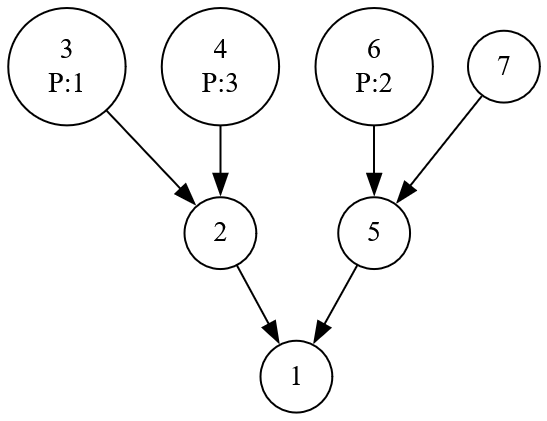
\includegraphics[width=0.3\textwidth]{sample.png}
    \\Each circle represents a house, and the arrows represent slides.
    The top number in each circle is the index of the house, and the bottom number is the index of the person living in the house (if any).
\end{figure}

The results of the queries are as follows:
\begin{itemize}
  \item In custom $1$, two people can be invited by inviting persons $1$ and $3$. The party can then be held in house $2$.
  However, it is not possible to invite persons $1$ and $2$, as no valid party house exists.
  \item In custom $2$, no more than person $2$ can be invited. Thus the party consists only of person $2$ in house $6$.
  \item In custom $3$, persons $2$ and $3$ swap houses.
  \item In custom $4$, it is now possible to host a party with persons $1$ and $2$ with party house $2$.
  \item In custom $5$, it is now possible to host a party with everyone if party house $1$ is chosen.
  \item In custom $6$, person $3$ moves to house $2$.
  \item In custom $7$, it is possible to host a party where everyone is invited with party house $2$.
\end{itemize}
